\documentclass[12pt,reqno]{amsart}
\usepackage{/Users/johnmyers/GoogleDrive/tex/handout,/Users/johnmyers/GoogleDrive/tex/customcommands,polynom}
\usepackage{caption}

\hdr{MAT 240}{\S17.3 Vector fields}

\begin{document}

\textbf{Suggested problems:} 1-27 odd, 31, 33

\bigskip
\hrule

\bigskip
\prob Sketch the following vector fields in $\bbr^2$.

\medskip
\begin{enumerate}
\item $\vec{F}(x,y) = \ang{2,3}$ \textcolor{red}{See class notes for sketch.}
\item $\vec{F}(x,y) = \ang{y,0}$ \textcolor{red}{See class notes for sketch.}
\item $\vec{F}(x,y) = \ang{ x,y}$ \textcolor{red}{See class notes for sketch.}
\item $\vec{F}(x,y) = \ang{ y,-x}$ \textcolor{red}{See class notes for sketch.}
\item $\vec{F}(x,y) = \displaystyle\frac{x\vec{i} + y\vec{j}}{\sqrt{x^2+y^2}}$ \textcolor{red}{See class notes for sketch.}
\end{enumerate}

\bigskip
\prob Match the vector fields in $\bbr^3$ to their formulas.

\bigskip
\begin{minipage}{0.3\textwidth}
\begin{enumerate}
\item $\vec{F}(x,y,z) = \ang{1,2,3}$ \textcolor{red}{IV}\vspace{0.5in}
\item $\vec{F}(x,y,z) = \ang{1,2,z}$ \\ \textcolor{red}{I}\vspace{0.5in}
\item $\vec{F}(x,y,z) = \ang{x,y,3}$ \textcolor{red}{III}\vspace{0.5in}
\item $\vec{F}(x,y,z) = \ang{x,y,z}$ \\ \textcolor{red}{II}
\end{enumerate}
\end{minipage}
\begin{minipage}{0.7\textwidth}
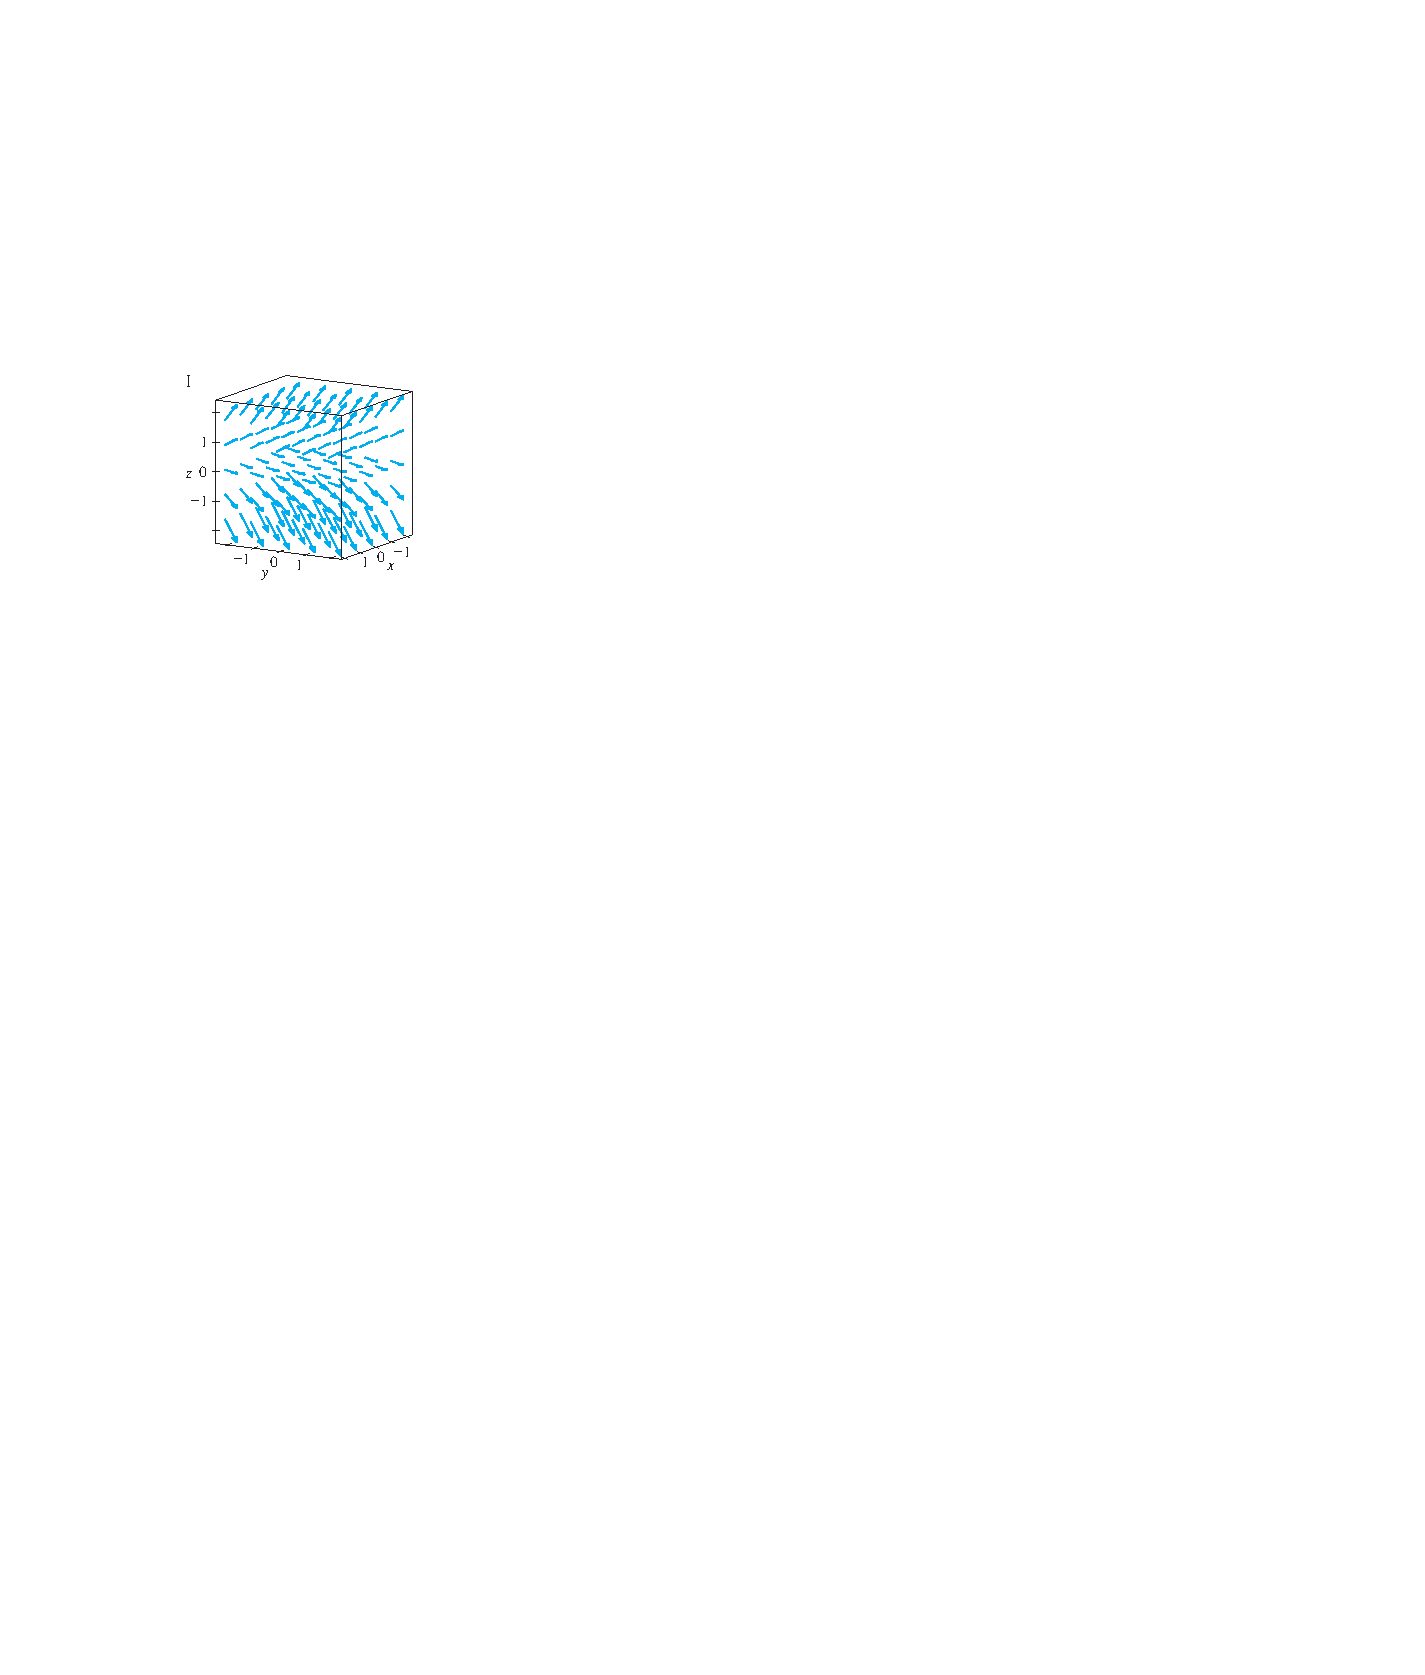
\includegraphics[scale=1.25]{I.pdf}

\includegraphics[scale=1.25]{II.pdf} \\

\includegraphics[scale=1.25]{III.pdf}
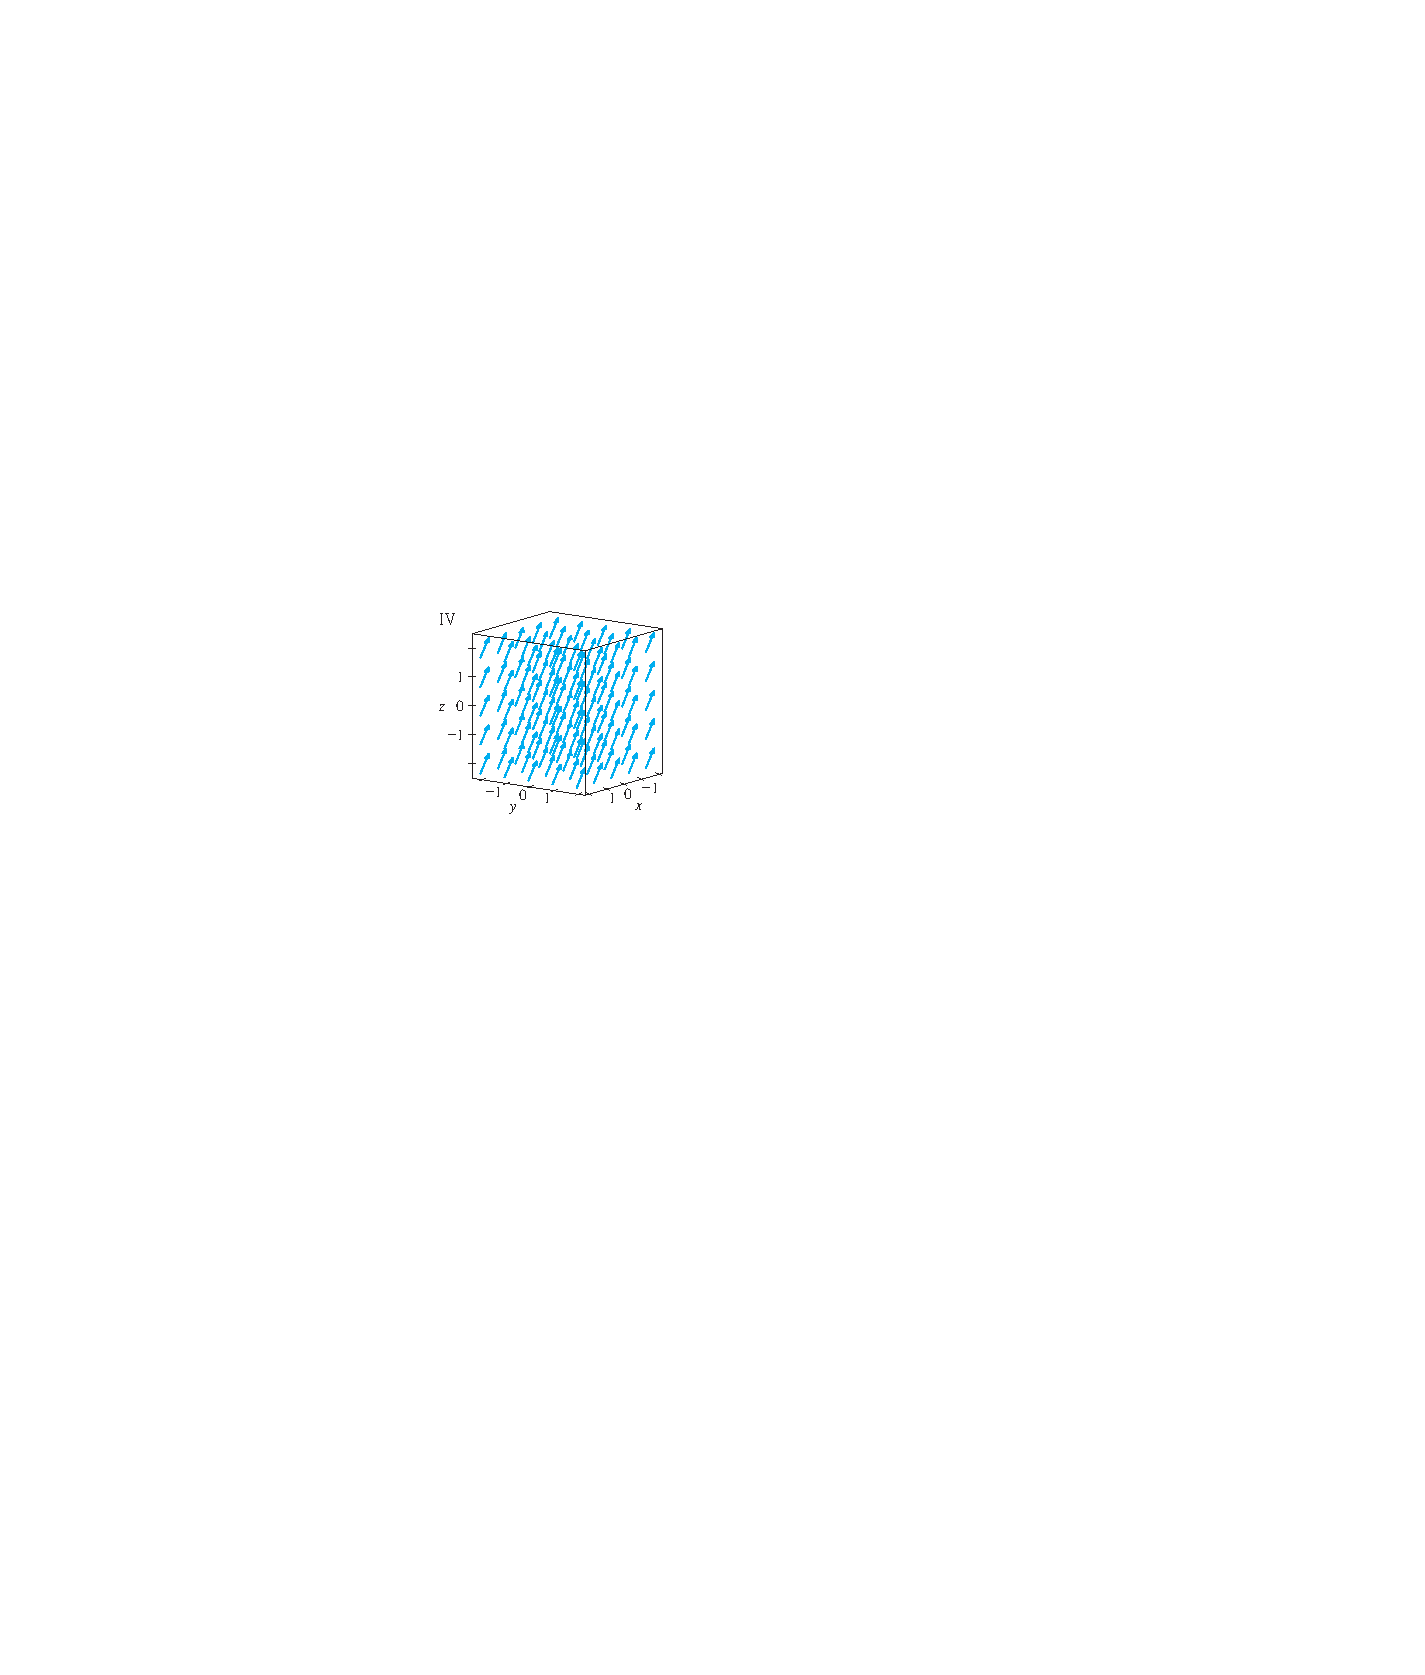
\includegraphics[scale=1.25]{IV.pdf}
\end{minipage}

\newpage
\prob Find formulas for the vectors fields below.

\bigskip
\begin{minipage}{0.5\textwidth}
\begin{itemize}
\item[(a)] \textcolor{white}{blank} \\

\includegraphics[scale=1.75]{pic1.pdf} \\ \textcolor{red}{$\vec{F}(x,y) = \ang{x,0}$}\vspace{0.5in}
\item[(c)] \textcolor{white}{blank} \\

\includegraphics[scale=1.75]{pic3.pdf} \\ \textcolor{red}{$\vec{F}(x,y) = \ang{x,y}$}\vspace{0.5in}
\item[(d)] \textcolor{white}{blank} \\

\includegraphics[scale=1.75]{pic4.pdf} \\ \textcolor{red}{$\vec{F}(x,y) = \ang{-y,x}$}
\end{itemize}
\end{minipage}
\begin{minipage}{0.5\textwidth}
\begin{itemize}
\item[(b)] \textcolor{white}{blank} \\

\includegraphics[scale=1.75]{pic2.pdf} \\ \textcolor{red}{$\vec{F}(x,y) = \ang{-y,0}$}\vspace{0.5in}
\item[(d)] \textcolor{white}{blank} \\

\includegraphics[scale=1.75]{pic5.pdf} \\ \textcolor{red}{$\vec{F}(x,y) = -\ang{x,y}$}\vspace{0.5in}
\item[(f)] \textcolor{white}{blank} \\

\includegraphics[scale=1.75]{pic6.pdf} \\ \textcolor{red}{$\vec{F}(x,y) = \frac{\ang{x,y}}{\sqrt{x^2+y^2}}$}
\end{itemize}
\end{minipage}

\newpage
\prob For each description of a vector field in parts (a)-(d), choose one or more of the vector fields (i)-(ix).

\bigskip
\begin{enumerate}
\item Pointing radially outward, increasing in length away from the origin. \textcolor{red}{iii}\vspace{0.5in}
\item Pointing in a circular direction around the origin, remaining the same length. \textcolor{red}{ii}\vspace{0.5in}
\item Pointing toward the origin, increasing in length farther from the origin. \textcolor{red}{iv}\vspace{0.5in}
\item Pointing clockwise around the origin. \textcolor{red}{vi}\vspace{0.5in}
\end{enumerate}

\begin{enumerate}[(i)]
\item $\displaystyle\frac{\ang{x,y}}{\sqrt{x^2+y^2}}$\bigskip
\item $\displaystyle\frac{\ang{-y,x}}{\sqrt{x^2+y^2}}$\bigskip
\item $x\vec{i} + y \vec{j}$\bigskip
\item $-x\vec{i} - y \vec{j}$\bigskip
\item $\ang{-y,x}$\bigskip
\item $\ang{y,-x}$\bigskip
\item $\ang{y,x}$\bigskip
\item $\displaystyle\frac{\ang{x,y}}{(x^2+y^2)^{3/2}}$\bigskip
\item $-\displaystyle\frac{\ang{x,y}}{(x^2+y^2)^{3/2}}$
\end{enumerate}

\newpage
\prob Match the contour plots in (a)-(d) with the gradient fields in (i)-(iv).

\medskip
\begin{minipage}{0.5\textwidth}
\begin{center}
\begin{enumerate}
\item\textcolor{white}{blank} \\

\includegraphics[scale=1.5]{pic11.pdf} \\ \textcolor{red}{iii}\vspace{0.5in}
\item\textcolor{white}{blank} \\

\includegraphics[scale=1.5]{pic12.pdf} \\ \textcolor{red}{ii}\vspace{0.5in}
\item\textcolor{white}{blank} \\

\includegraphics[scale=1.5]{pic13.pdf}  \\ \textcolor{red}{iv}\vspace{0.5in}
\item\textcolor{white}{blank} \\

\includegraphics[scale=1.5]{pic14.pdf} \\ \textcolor{red}{i}
\end{enumerate}
\end{center}
\end{minipage}\begin{minipage}{0.5\textwidth}
\begin{center}
\begin{enumerate}[(i)]
\item\textcolor{white}{blank} \\

\includegraphics[scale=1.5]{pic15.pdf}\vspace{0.5in}
\item\textcolor{white}{blank} \\

\includegraphics[scale=1.5]{pic16.pdf}\vspace{0.5in}
\item\textcolor{white}{blank} \\

\includegraphics[scale=1.5]{pic17.pdf}\vspace{0.5in}
\item\textcolor{white}{blank} \\

\includegraphics[scale=1.5]{pic18.pdf}
\end{enumerate}
\end{center}
\end{minipage}



\end{document}